\documentclass[preview]{standalone}

\usepackage{amsmath}
\usepackage{amssymb}
\usepackage{tikz}
\usepackage{stellar}
\usepackage{definitions}
\usepackage{bettelini}

\begin{document}

\id{linearalgebra-affine-subspaces}
\genpage

\section{Affine subspaces}

\begin{snippetdefinition}{affine-subspace-definition}{Affine subspace}
    Let \(\mathcal{A}\) be an \affinespace over a \field
    \(\mathbb{F}\), with associated \vectorspace \(V\). A \set
    \(U\subseteq\mathcal{A}\) is an \emph{affine subspace} if
    \(U=\emptyset\), or if there exists \(p\in U\) such that
    \[
        \vec{U}_p
        =
        \{\vec{pq}\suchthat q\in U\}
    \]
    is a linear subspace of \(V\). In this case \(\vec{U}_p\) is called
    the \emph{direction} of \(U\).
\end{snippetdefinition}

\begin{snippetproposition}{affine-subspace-direction-well-defined}{The direction is well-defined}
    Let \(\mathcal{A}\) be an \affinespace over a \field
    \(\mathbb{F}\), with associated \vectorspace \(V\). Let
    \(U\subseteq\mathcal{A}\) be nonempty. If there exists \(p\in U\) such
    that
    \[
        \vec{U}_p=\{\vec{pq}\suchthat q\in U\}
    \]
    is a linear subspace of \(V\), then for every \(r\in U\),
    \[
        \vec{U}_r=\{\vec{rq}\suchthat q\in U\}
    \]
    is the same linear subspace. Therefore the direction of \(U\) does not
    depend on the chosen point.
\end{snippetproposition}

\begin{snippetproof}{affine-subspace-direction-well-defined-proof}{affine-subspace-direction-well-defined}{The direction is well-defined}
    Let \(r\in U\). Since \(r\in U\), we have
    \(\vec{pr}\in\vec{U}_p\). If \(q\in U\), then by Chasles
    \[
        \vec{rq}=\vec{rp}+\vec{pq}.
    \]
    Both \(\vec{rp}=-\vec{pr}\) and \(\vec{pq}\) belong to
    \(\vec{U}_p\), so \(\vec{rq}\in\vec{U}_p\). Hence
    \[
        \vec{U}_r\subseteq\vec{U}_p.
    \]

    Conversely, let \(u\in\vec{U}_p\). Since
    \(\vec{pr}+u\in\vec{U}_p\), there exists \(s\in U\) such that
    \[
        \vec{ps}=\vec{pr}+u.
    \]
    Then
    \[
        \vec{rs}
        =
        \vec{rp}+\vec{ps}
        =
        -\vec{pr}+(\vec{pr}+u)
        =
        u.
    \]
    Thus \(u\in\vec{U}_r\), so \(\vec{U}_p\subseteq\vec{U}_r\).
\end{snippetproof}

\begin{snippetdefinition}{affine-subspace-dimension-definition}{Dimension of an affine subspace}
    Let \(U\) be a nonempty affine subspace of an \affinespace, with
    direction \(\vec{U}\). The \emph{dimension} of \(U\) is
    \[
        \lineardim(U)\triangleq\lineardim(\vec{U}).
    \]
    By convention, \(\lineardim(\emptyset)=-\infty\).
\end{snippetdefinition}

\section{Examples}

\begin{snippetexample}{translated-subspaces-affine-subspaces-example}{Translated subspaces}
    Let \(\mathcal{A}\) be an \affinespace over a \field
    \(\mathbb{F}\), with associated \vectorspace \(V\). Let
    \(W\subseteq V\) be a linear subspace and let \(p\in\mathcal{A}\).
    Then
    \[
        p+W
        =
        \{q\in\mathcal{A}\suchthat\vec{pq}\in W\}
    \]
    is an affine subspace of \(\mathcal{A}\) with direction \(W\).
\end{snippetexample}

\begin{snippetexample}{points-lines-planes-affine-subspaces-example}{Points, lines and planes}
    Let \(U\) be a nonempty affine subspace of an \affinespace.
    If
    \[
        \lineardim(U)=0,
    \]
    then \(U\) is a point. If
    \[
        \lineardim(U)=1,
    \]
    then \(U\) is an affine line. If
    \[
        \lineardim(U)=2,
    \]
    then \(U\) is an affine plane.
\end{snippetexample}

\begin{snippetexample}{affine-line-a2-cartesian-example}{An affine line in \(\mathbb{A}^2(\mathbb{R})\)}
    In \(\mathbb{A}^2(\realnumbers)\), let
    \[
        U=\{(x,y)\in\mathbb{A}^2(\realnumbers)\suchthat 2x+3y-6=0\}.
    \]
    Then \(U\) is an affine line. Since
    \[
        (3,0)\in U,
        \qquad
        (0,2)\in U,
    \]
    its direction is generated by the \vector
    \[
        (3,0)-(0,2)=(3,-2).
    \]
    Hence
    \[
        \vec{U}=\linearspan((3,-2)).
    \]
    \[
        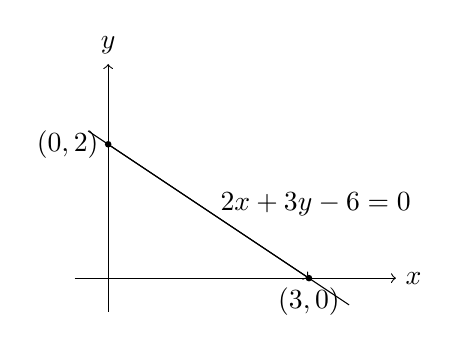
\begin{tikzpicture}[scale=0.85]
            \draw[->] (-0.5,0) -- (4.3,0) node[right] {\(x\)};
            \draw[->] (0,-0.5) -- (0,3.2) node[above] {\(y\)};
            \draw (-0.3,2.2) -- (3.6,-0.4);
            \fill (0,2) circle (1.4pt) node[left] {\((0,2)\)};
            \fill (3,0) circle (1.4pt) node[below] {\((3,0)\)};
            \draw[->] (0,2) -- (3,0);
            \node at (3.1,1.1) {\(2x+3y-6=0\)};
        \end{tikzpicture}
    \]
\end{snippetexample}

\begin{snippetproposition}{affine-subspace-intersection}{Intersection of affine subspaces}
    Let \(\mathcal{A}\) be an \affinespace. The intersection of any family
    of affine subspaces of \(\mathcal{A}\) is an affine subspace of
    \(\mathcal{A}\).
\end{snippetproposition}

\begin{snippetproof}{affine-subspace-intersection-proof}{affine-subspace-intersection}{Intersection of affine subspaces}
    If the intersection is empty, it is an affine subspace by definition.
    Otherwise, let
    \[
        p\in\bigcap_{i\in I}U_i.
    \]
    Then
    \[
        \left\{\vec{pq}\suchthat q\in\bigcap_{i\in I}U_i\right\}
        =
        \bigcap_{i\in I}
        \{\vec{pq}\suchthat q\in U_i\}.
    \]
    Each \(\{\vec{pq}\suchthat q\in U_i\}\) is a linear subspace of the direction
    \vectorspace, and intersections of linear subspaces are linear
    subspaces. Therefore \(\bigcap_{i\in I}U_i\) is an affine subspace.
\end{snippetproof}

\section{Affine span}

\begin{snippetdefinition}{affine-span-definition}{Affine span}
    Let \(\mathcal{A}\) be an \affinespace and let
    \(S\subseteq\mathcal{A}\). The \emph{affine span} of \(S\), denoted
    \[
        \operatorname{Aff}(S),
    \]
    is the intersection of all affine subspaces of \(\mathcal{A}\)
    containing \(S\). Equivalently, it is the smallest affine subspace of
    \(\mathcal{A}\) containing \(S\).
\end{snippetdefinition}

\begin{snippetproposition}{finite-affine-span-description}{Affine span of finitely many points}
    Let \(\mathcal{A}\) be an \affinespace over a \field
    \(\mathbb{F}\), and let
    \[
        S=\{p_0,p_1,\ldots,p_k\}\subseteq\mathcal{A}.
    \]
    Then
    \[
        \operatorname{Aff}(S)
        =
        p_0+
        \linearspan(\vec{p_0p_1},\ldots,\vec{p_0p_k}).
    \]
    In particular,
    \[
        \lineardim\operatorname{Aff}(p_0,\ldots,p_k)\leq k.
    \]
\end{snippetproposition}

\begin{snippetproof}{finite-affine-span-description-proof}{finite-affine-span-description}{Affine span of finitely many points}
    The \set
    \[
        p_0+
        \linearspan(\vec{p_0p_1},\ldots,\vec{p_0p_k})
    \]
    is an affine subspace containing every \(p_i\). If \(U\) is any affine
    subspace containing \(p_0,\ldots,p_k\), then its direction contains
    \[
        \vec{p_0p_1},\ldots,\vec{p_0p_k}.
    \]
    Therefore it contains their \linearspantext, and hence contains
    \(p_0+\linearspan(\vec{p_0p_1},\ldots,\vec{p_0p_k})\). This proves
    minimality.
\end{snippetproof}

\begin{snippetdefinition}{affine-independence-definition}{Affine independence}
    Let \(\mathcal{A}\) be an \affinespace. The
    \affinepoint[points]
    \[
        p_0,\ldots,p_k\in\mathcal{A}
    \]
    are \emph{affinely independent} if
    \[
        \lineardim\operatorname{Aff}(p_0,\ldots,p_k)=k.
    \]
    Equivalently,
    \[
        \vec{p_0p_1},\ldots,\vec{p_0p_k}
    \]
    are \linearlyindependent in the direction \vectorspace of
    \(\mathcal{A}\).
\end{snippetdefinition}

\begin{snippetexample}{affine-independent-points-a2-example}{Three points in the affine plane}
    In \(\mathbb{A}^2(\realnumbers)\), three
    \affinepoint[points] are \affinelyindependent if and only if they are
    not collinear.
    \[
        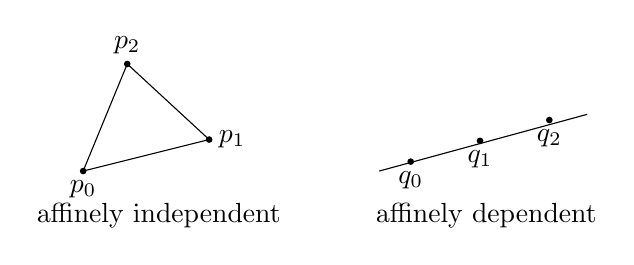
\begin{tikzpicture}[scale=0.8]
            \fill (0,0) circle (1.5pt) node[below] {\(p_0\)};
            \fill (2,0.5) circle (1.5pt) node[right] {\(p_1\)};
            \fill (0.7,1.7) circle (1.5pt) node[above] {\(p_2\)};
            \draw (0,0) -- (2,0.5) -- (0.7,1.7) -- cycle;
            \node at (1.2,-0.7) {affinely independent};
            \begin{scope}[xshift=5cm]
                \draw (-0.3,0) -- (3,0.9);
                \fill (0.2,0.15) circle (1.5pt) node[below] {\(q_0\)};
                \fill (1.3,0.48) circle (1.5pt) node[below] {\(q_1\)};
                \fill (2.4,0.81) circle (1.5pt) node[below] {\(q_2\)};
                \node at (1.4,-0.7) {affinely dependent};
            \end{scope}
        \end{tikzpicture}
    \]
\end{snippetexample}

\section{Affine frames}

\begin{snippetdefinition}{affine-frame-definition}{Affine frame}
    Let \(\mathcal{A}\) be an \(n\)-dimensional \affinespace over a
    \field \(\mathbb{F}\). An \emph{affine frame} of \(\mathcal{A}\) is an
    ordered collection of \affinelyindependent \affinepoint[points]
    \[
        (p_0,p_1,\ldots,p_n).
    \]
    Equivalently,
    \[
        \{\vec{p_0p_1},\ldots,\vec{p_0p_n}\}
    \]
    is a \basis of the direction \vectorspace of \(\mathcal{A}\). The
    point \(p_0\) is the origin of the frame.
\end{snippetdefinition}

\begin{snippetdefinition}{affine-frame-coordinates-definition}{Coordinates in an affine frame}
    Let \(\mathcal{A}\) be an \(n\)-dimensional \affinespace over a
    \field \(\mathbb{F}\), and let
    \[
        (p_0,p_1,\ldots,p_n)
    \]
    be an \affineframe of \(\mathcal{A}\). For every
    \(q\in\mathcal{A}\), there exist unique
    \(\alpha_1,\ldots,\alpha_n\in\mathbb{F}\) such that
    \[
        \vec{p_0q}
        =
        \alpha_1\vec{p_0p_1}
        +\cdots+
        \alpha_n\vec{p_0p_n}.
    \]
    The tuple
    \[
        (\alpha_1,\ldots,\alpha_n)
    \]
    is called the coordinate tuple of \(q\) with respect to the affine
    frame.
\end{snippetdefinition}

\begin{snippetdefinition}{canonical-affine-frame-definition}{Canonical affine frame}
    In \(\mathbb{A}^n(\mathbb{F})\), the affine frame
    \[
        (0,e_1,\ldots,e_n)
    \]
    is called the \emph{canonical affine frame}.
\end{snippetdefinition}

\begin{snippetexample}{affine-frame-a2-coordinate-example}{Coordinates in an affine frame of \(\mathbb{A}^2(\mathbb{R})\)}
    In \(\mathbb{A}^2(\realnumbers)\), let
    \[
        p_0=(1,1),
        \qquad
        p_1=(3,5),
        \qquad
        p_2=(2,7).
    \]
    Then
    \[
        \vec{p_0p_1}=(2,4),
        \qquad
        \vec{p_0p_2}=(1,6).
    \]
    These two \vector[vectors] are \linearlyindependent because
    \[
        \det
        \begin{pmatrix}
            2 & 1\\
            4 & 6
        \end{pmatrix}
        =
        8\neq0.
    \]
    Thus \((p_0,p_1,p_2)\) is an \affineframe.

    For \(q=(0,0)\), the coordinates \((\alpha,\beta)\) satisfy
    \[
        (-1,-1)=\alpha(2,4)+\beta(1,6).
    \]
    Solving gives
    \[
        \alpha=-\frac{5}{8},
        \qquad
        \beta=\frac{1}{4}.
    \]
\end{snippetexample}

\section{Equations}

\begin{snippetdefinition}{affine-subspace-parametric-equations}{Parametric equations}
    Let \(\mathcal{A}\) be a \(k\)-dimensional \affinespace with a fixed
    \affineframe, and let \(U\subseteq\mathcal{A}\) be a nonempty affine
    subspace. Let \(r\in U\), and let
    \[
        \{v_1,\ldots,v_m\}
    \]
    be a \basis of the direction \(\vec{U}\). In coordinates, if
    \[
        r=(r_1,\ldots,r_k),
        \qquad
        v_i=(v_i^1,\ldots,v_i^k),
    \]
    then every point \(q=(x_1,\ldots,x_k)\in U\) has the form
    \[
        q=r+\alpha_1v_1+\cdots+\alpha_mv_m,
        \qquad
        \alpha_1,\ldots,\alpha_m\in\mathbb{F}.
    \]
    Equivalently,
    \[
        x_j=r_j+\alpha_1v_1^j+\cdots+\alpha_mv_m^j,
        \qquad
        j=1,\ldots,k.
    \]
\end{snippetdefinition}

\begin{snippetexample}{affine-line-a3-parametric-example}{Parametric equations of a line in \(\mathbb{A}^3(\mathbb{R})\)}
    In \(\mathbb{A}^3(\realnumbers)\) with the canonical affine frame,
    let \(U\) be the affine line through
    \[
        p=(1,1,1)
    \]
    with direction
    \[
        \linearspan((2,3,5)).
    \]
    Then
    \[
        U=p+\linearspan((2,3,5)),
    \]
    and its parametric equations are
    \[
        \begin{cases}
            x_1=1+2t,\\
            x_2=1+3t,\\
            x_3=1+5t,
        \end{cases}
        \qquad
        t\in\realnumbers.
    \]
\end{snippetexample}

\begin{snippetdefinition}{affine-subspace-cartesian-equations}{Cartesian equations}
    Let \(\mathcal{A}\) be a \(k\)-dimensional \affinespace with a fixed
    \affineframe, and let \(U\subseteq\mathcal{A}\) be a nonempty affine
    subspace. Suppose that the direction \(\vec{U}\subseteq\mathbb{F}^k\)
    is described by homogeneous equations
    \[
        a_{i1}x_1+\cdots+a_{ik}x_k=0,
        \qquad
        i=1,\ldots,m.
    \]
    If \(r=(r_1,\ldots,r_k)\in U\), then a point
    \(y=(y_1,\ldots,y_k)\) belongs to \(U\) if and only if
    \[
        a_{i1}(y_1-r_1)+\cdots+a_{ik}(y_k-r_k)=0,
        \qquad
        i=1,\ldots,m.
    \]
    Equivalently,
    \[
        a_{i1}y_1+\cdots+a_{ik}y_k=b_i,
        \qquad
        b_i=a_{i1}r_1+\cdots+a_{ik}r_k.
    \]
\end{snippetdefinition}

\begin{snippetexample}{affine-line-a3-cartesian-example}{Cartesian equations of the same line}
    In \(\mathbb{A}^3(\realnumbers)\), let
    \[
        p=(1,1,1),
        \qquad
        v=(2,3,5).
    \]
    The direction \(\linearspan(v)\) is described by
    \[
        3x_1-2x_2=0,
        \qquad
        5x_1-2x_3=0.
    \]
    Therefore the affine line \(p+\linearspan(v)\) is described by
    \[
        \begin{cases}
            3(y_1-1)-2(y_2-1)=0,\\
            5(y_1-1)-2(y_3-1)=0.
        \end{cases}
    \]
    Equivalently,
    \[
        \begin{cases}
            3y_1-2y_2=1,\\
            5y_1-2y_3=3.
        \end{cases}
    \]
\end{snippetexample}

\section{Parallelism}

\begin{snippetdefinition}{parallel-affine-spaces-definition}{Parallel affine subspaces}
    Let \(\mathcal{A}\) be an \affinespace, and let
    \(U,W\subseteq\mathcal{A}\) be nonempty affine subspaces. The subspaces
    \(U\) and \(W\) are \emph{parallel} if they have the same direction:
    \[
        \vec{U}=\vec{W}.
    \]
    In this case we write
    \[
        U\parallel W.
    \]
\end{snippetdefinition}

\begin{snippetexample}{parallel-affine-lines-a3-example}{Two parallel lines in \(\mathbb{A}^3(\mathbb{R})\)}
    In \(\mathbb{A}^3(\realnumbers)\), let
    \[
        \ell:
        \begin{cases}
            x=3-t,\\
            y=2+t,\\
            z=1-2t,
        \end{cases}
        \qquad
        t\in\realnumbers.
    \]
    Then
    \[
        \vec{\ell}=\linearspan((-1,1,-2)).
    \]
    Let
    \[
        \ell'
        =
        \left\{
            (x,y,z)\in\mathbb{A}^3(\realnumbers)
            \suchthat
            x+y=5,\ x-y-z=7
        \right\}.
    \]
    The associated homogeneous system is
    \[
        x+y=0,
        \qquad
        x-y-z=0.
    \]
    Its solutions are \((x,-x,2x)=x(1,-1,2)\). Hence
    \[
        \vec{\ell'}=\linearspan((1,-1,2))=\vec{\ell},
    \]
    so \(\ell\parallel\ell'\).
\end{snippetexample}

\begin{snippetexample}{linear-system-solution-spaces-parallel-example}{Linear systems with different constant terms}
    Let \(\mathbb{F}\) be a \field, let
    \(A\in\matrices_{m\times n}(\mathbb{F})\), and let
    \(b,c\in\mathbb{F}^m\). If the solution \set[sets]
    \[
        S_b=\{x\in\mathbb{F}^n\suchthat Ax=b\},
        \qquad
        S_c=\{x\in\mathbb{F}^n\suchthat Ax=c\}
    \]
    are nonempty, then they are affine subspaces of
    \(\mathbb{A}^n(\mathbb{F})\) with the same direction \(\ker A\).
    Therefore
    \[
        S_b\parallel S_c.
    \]
\end{snippetexample}

\begin{snippetproposition}{parallel-affine-spaces-either-disjoint-or-same}{Parallel affine subspaces are disjoint or equal}
    Let \(\mathcal{A}\) be an \affinespace, and let
    \(U,W\subseteq\mathcal{A}\) be parallel affine subspaces. Then
    \[
        U\intersection W=\emptyset
        \qquad
        \text{or}
        \qquad
        U=W.
    \]
\end{snippetproposition}

\begin{snippetproof}{parallel-affine-spaces-either-disjoint-or-same-proof}{parallel-affine-spaces-either-disjoint-or-same}{Parallel affine subspaces are disjoint or equal}
    Suppose that \(U\intersection W\neq\emptyset\), and let
    \(p\in U\intersection W\). Since \(U\parallel W\), we have
    \[
        \vec{U}=\vec{W}.
    \]
    If \(q\in U\), then \(\vec{pq}\in\vec{U}=\vec{W}\). Since
    \(p\in W\), this implies \(q\in W\). Hence \(U\subseteq W\). The same
    argument with \(U\) and \(W\) exchanged gives \(W\subseteq U\), so
    \(U=W\).
\end{snippetproof}

\begin{snippetproposition}{affine-spaces-fifth-postulate}{Parallel postulate in an affine plane}
    Let \(\mathcal{P}\) be an affine plane over a \field
    \(\mathbb{F}\). Let \(\ell\subseteq\mathcal{P}\) be an affine line and
    let \(p\in\mathcal{P}\). Then there exists a unique affine line through
    \(p\) parallel to \(\ell\).
\end{snippetproposition}

\begin{snippetproof}{affine-spaces-fifth-postulate-proof}{affine-spaces-fifth-postulate}{Parallel postulate in an affine plane}
    Let \(L=\vec{\ell}\) be the direction of \(\ell\). Define
    \[
        \ell'
        =
        p+L
        =
        \{q\in\mathcal{P}\suchthat\vec{pq}\in L\}.
    \]
    Then \(\ell'\) is an affine line through \(p\), and
    \(\vec{\ell'}=L=\vec{\ell}\), so \(\ell'\parallel\ell\).

    If \(m\) is another affine line through \(p\) parallel to \(\ell\),
    then \(\vec{m}=\vec{\ell}=L\). Since \(p\in m\), we have
    \(m=p+L=\ell'\). Hence \(\ell'\) is unique.
\end{snippetproof}

\section{Thales theorem}

\begin{snippet}{affine-thales-diagram}
    \[
        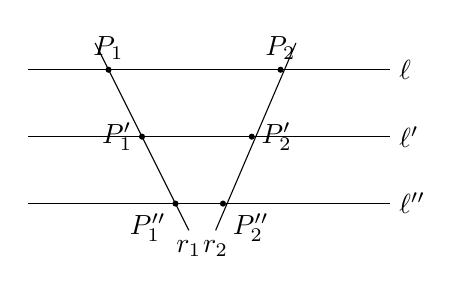
\begin{tikzpicture}[scale=0.85]
            \draw (-0.2,3) -- (5.2,3) node[right] {\(\ell\)};
            \draw (-0.2,2) -- (5.2,2) node[right] {\(\ell'\)};
            \draw (-0.2,1) -- (5.2,1) node[right] {\(\ell''\)};
            \draw (0.8,3.4) -- (2.2,0.6) node[below] {\(r_1\)};
            \draw (3.8,3.4) -- (2.6,0.6) node[below] {\(r_2\)};
            \fill (1.0,3) circle (1.3pt) node[above] {\(P_1\)};
            \fill (1.5,2) circle (1.3pt) node[left] {\(P_1'\)};
            \fill (2.0,1) circle (1.3pt) node[below left] {\(P_1''\)};
            \fill (3.57,3) circle (1.3pt) node[above] {\(P_2\)};
            \fill (3.14,2) circle (1.3pt) node[right] {\(P_2'\)};
            \fill (2.71,1) circle (1.3pt) node[below right] {\(P_2''\)};
        \end{tikzpicture}
    \]
\end{snippet}

\begin{snippettheorem}{talete-theorem}{Affine Thales theorem}
    Let \(\mathcal{P}\) be an affine plane over a \field \(\mathbb{F}\).
    Let
    \[
        \ell,\ell',\ell''
    \]
    be three distinct parallel affine lines in \(\mathcal{P}\), and let
    \(r_1,r_2\) be affine lines not parallel to them. For \(i=1,2\), set
    \[
        P_i=r_i\intersection\ell,
        \qquad
        P_i'=r_i\intersection\ell',
        \qquad
        P_i''=r_i\intersection\ell''.
    \]
    If \(k_1,k_2\in\mathbb{F}\) satisfy
    \[
        \vec{P_1P_1''}=k_1\vec{P_1P_1'},
        \qquad
        \vec{P_2P_2''}=k_2\vec{P_2P_2'},
    \]
    then
    \[
        k_1=k_2.
    \]
\end{snippettheorem}

\begin{snippetproof}{talete-theorem-proof}{talete-theorem}{Affine Thales theorem}
    If \(r_1=r_2\), the statement is immediate. Suppose \(r_1\neq r_2\).
    By possibly exchanging the parallel lines, we may assume
    \(P_1\neq P_2\). Put
    \[
        v=\vec{P_1P_2}\neq0.
    \]
    Since \(\ell\parallel\ell'\), the \vector[vectors]
    \(\vec{P_1P_2}\) and \(\vec{P_1'P_2'}\) belong to the same one
    dimensional direction. Hence there exists \(\alpha\in\mathbb{F}\) such
    that
    \[
        \vec{P_2P_2'}-\vec{P_1P_1'}=\alpha v.
    \]
    Similarly, since \(\ell\parallel\ell''\), there exists
    \(\beta\in\mathbb{F}\) such that
    \[
        \vec{P_2P_2''}-\vec{P_1P_1''}=\beta v.
    \]

    If \(\alpha=0\), then
    \[
        \vec{P_2P_2'}=\vec{P_1P_1'}.
    \]
    The same parallelogram argument with \(\ell\) and \(\ell''\) gives
    \[
        \vec{P_2P_2''}=\vec{P_1P_1''}.
    \]
    Since the lines \(r_1\) and \(r_2\) are not parallel to the three
    parallel lines, the \vector[vectors] \(\vec{P_iP_i'}\) are nonzero.
    Therefore
    \[
        k_1=k_2.
    \]

    Suppose now that \(\alpha\neq0\). The \vector[vectors]
    \(\vec{P_1P_1'}\) and \(\vec{P_2P_2'}\) are \linearlyindependent.
    Indeed, if they were dependent, then
    \(\vec{P_2P_2'}-\vec{P_1P_1'}\) would lie in the direction of one of
    the \(r_i\). Since this difference is \(\alpha v\) with
    \(\alpha\neq0\), the direction of \(r_i\) would equal the direction of
    the parallel lines, contradicting the hypotheses.

    From
    \[
        \vec{P_2P_2'}-\vec{P_1P_1'}=\alpha v
    \]
    we get
    \[
        v=
        \alpha^{-1}
        \left(
            \vec{P_2P_2'}-\vec{P_1P_1'}
        \right).
    \]
    Using the hypotheses and
    \(\vec{P_2P_2''}-\vec{P_1P_1''}=\beta v\), we obtain
    \[
        k_2\vec{P_2P_2'}-k_1\vec{P_1P_1'}
        =
        \alpha^{-1}\beta
        \left(
            \vec{P_2P_2'}-\vec{P_1P_1'}
        \right).
    \]
    Hence
    \[
        \left(k_2-\alpha^{-1}\beta\right)\vec{P_2P_2'}
        +
        \left(\alpha^{-1}\beta-k_1\right)\vec{P_1P_1'}
        =
        0.
    \]
    By linear independence, both coefficients are zero. Therefore
    \[
        k_1=\alpha^{-1}\beta=k_2.
    \]
\end{snippetproof}

\end{document}
